\documentclass[a4paper,12pt]{article}
\usepackage[utf8]{inputenc}
\usepackage[T1]{fontenc}
\usepackage[spanish]{babel}
\usepackage{csquotes}
\usepackage{anysize}
\usepackage{graphicx}
\usepackage{hyperref}
\usepackage{pgfplots}
\pgfplotsset{compat=1.18}
%\usepackage{amsfonts}
%\usepackage{tikz}
%\usepackage{amsmath}
\marginsize{25mm}{25mm}{25mm}{25mm}

\title{Estadística inferencial}
\author{Daniel Maldonado}
\date{}

\begin{document}
{\scshape\bfseries \maketitle}

\section{Prueba de hipótesis}\label{pruebahipotesis}

La estadística inferencial permite generalizar los resultados de muestras hacia poblaciones con niveles razonables de confianza. Esto se realiza mediante pruebas de hipótesis.

Una hipótesis experimental podría ser que la media $\bar{X}$ del grupo al cual se aplicó una intervención es distinta de la media $\mu$ de la población de la cual se obtuvo la muestra. Es decir,
\begin{eqnarray*}
  \bar{X} &<& \mu\\
          &\mbox{o}&\\
  \bar{X} &>& \mu,
\end{eqnarray*}
o de forma más general:
\[
  \bar{X} \neq \mu
.\]

Suponemos que la muestra tenía originalmente la misma media que la población, y que la aplicación de nuestra intervención desplazó su media en una cierta dirección. En cierto modo, suponemos que nuestra intervención tiene el efecto de crear una segunda población con una media distinta de la población original.

Si la muestra fuese perfectamente representativa de la población original, entonces se podría concluir que, si la media muestral $\bar{X}$ después del tratamiento es distinta de la media de la población $\mu$, entonces el tratamiento es eficaz. Sin embargo, la realidad no suele ser tan bella.

Una amenaza seria a la validez de la relación encontrada entre la aplicación del tratamiento experimental y el cambio en la media de la muestra es la posibilidad de un error de muestreo, es decir, que por azar la media de la muestra no fuese representativa de la población desde el comienzo. Esto tiene base en el {\slshape teorema central del límite} o {\slshape teorema del límite central}.

De acuerdo con el teorema podemos obtener muestras de una población y calcular la media de cada una de esas muestras. Si la cantidad de medias es lo bastante grande, entonces la distribución de esas medias tenderá a ser normal (una campana de Gauss) y la media formada por estas medias muestrales será muy cercana a la media $\mu$ de la población. Sin embargo, aunque las medias de las muestras tenderán a rondar el valor de la media poblacional, habrá una minoría que se encuentre muy lejos, ya sea por encima o por debajo. Así, existe una probabilidad nada despreciable de que la media de la muestra obtenida de la población esté muy por encima o muy por debajo del valor poblacional (Figura 1).

\begin{figure}[!ht]
  \begin{center}
    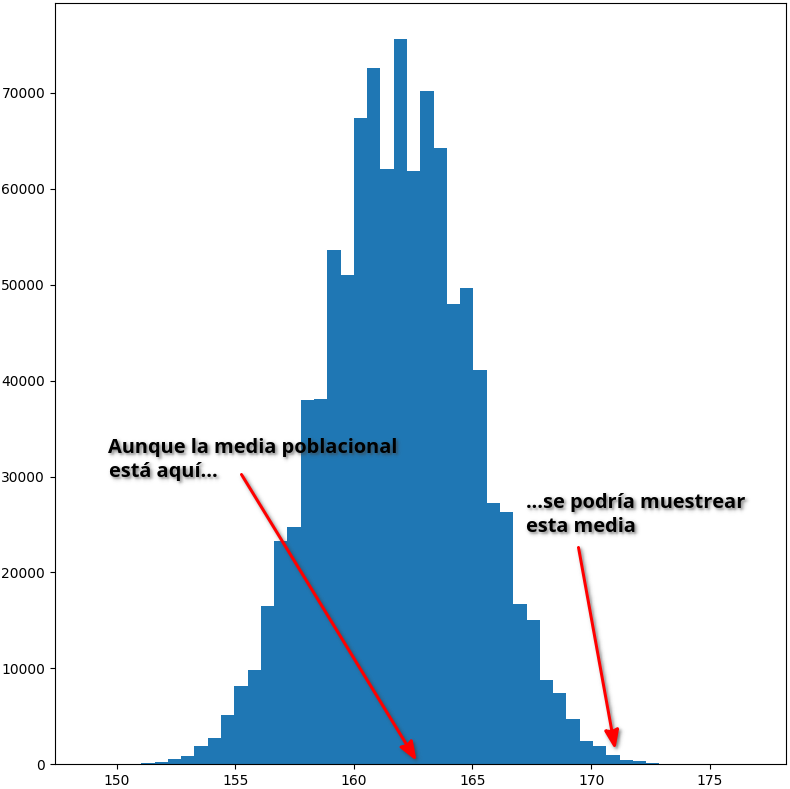
\includegraphics[scale=0.5]{curvaNormal.png}
    \caption{La media de la muestra puede estar en cualquier punto de la distribución.}
  \end{center}
\end{figure}

Si este fuera el caso, entonces la diferencia que encontramos entre la media $\bar{X}$ de la muestra tras el tratamiento y la media de la población $\mu$ sería solo debida al azar.

El papel de la estadística inferencial es garantizar que no cometamos el error de atribuir a la variable independiente (el tratamiento) las diferencias debidas a un error de muestreo. ¿Concluimos que la relación encontrada en la muestra se cumpliría si evaluamos a toda la población, o concluimos que es una coincidencia debida al error?

El procedimiento estadístico específico a usar dependerá del diseño experimental y la hipótesis, pero de modo general se puede utilizar estadística {\itshape paramétrica} y {\itshape no paramétrica}.

La estadística paramétrica requiere que se cumplan ciertos supuestos dentro de los datos de la muestra:
\begin{itemize}
  \item La población de puntuaciones de la variable dependiente forma una distribución normal (o aproximadamente normal)
  \item Las puntuaciones tienen nivel de medición de intervalos o de razón
\end{itemize}

La estadística paramétrica suele ser preferible, así que se utiliza a menos que haya flagrantes violaciones de los supuestos que tiene.

De forma general los pasos para las pruebas de hipótesis son
\begin{enumerate}
  \item Establecer una hipótesis experimental
  \item Diseñar y correr un experimento que permita probarla
  \item Traducir la hipótesis experimental en una hipótesis estadística
  \item Seleccionar y llevar a cabo el procedimiento estadístico correcto para probarla
\end{enumerate}

Las hipótesis generalmente dirán cosas similares a ``{\slshape a incrementos en X corresponden incrementos en Y}'', o ``{\slshape a incrementos en X corresponden disminuciones en Y}'', es decir, habrá una relación ordenada entre las variables, y esa relación tendrá una dirección positiva o negativa.

Si la relación es positiva, esto significará que esperamos que la media de la muestra después del tratamiento esté a la {\slshape derecha} de la media poblacional. Si la hipótesis es correcta entonces esta media muestral caerá en un punto lo bastante alejado de la media poblacional para poder decir con razonables niveles de confianza que no pertenece a la misma distribución, sino que pertenece a una nueva distribución creada por la intervención.

El punto de corte estándar en psicología es el percentil 95 de la distribución poblacional. Es decir, si la media de la muestra cae en la cola derecha de la distribución poblacional en un punto tan alejado de la media que menos del 5\% de las ocasiones en que se muestree esa distribución aparecerá un valor así de elevado, entonces tendremos suficiente certeza de que la intervención es eficaz y efectivamente desplaza los puntajes hacia la derecha.

Si anticipamos una relación negativa, ocurre lo mismo pero hacia el lado izquierdo de la distribución. Si anticipamos que habrá un cambio, pero no sabemos en qué dirección, entonces el punto de corte de 5\% se repartirá entre las dos colas de la distribución, 2.5\% de cada lado. Esta es la diferencia entre pruebas de ``una cola'' y de ``dos colas''.

\pgfmathdeclarefunction{gauss}{2}{%
  \pgfmathparse{1/(#2*sqrt(2*pi))*exp(-((x-#1)^2)/(2*#2^2))}%
}

\begin{figure}[!ht]
  \begin{center}
    \begin{tikzpicture}
      \begin{axis}[
        no markers, domain=-5:5, samples=100,
        axis lines*=left, xlabel=$x$, ylabel=$\bar{X}$,
        every axis y label/.style={at=(current axis.above origin),anchor=south},
        every axis x label/.style={at=(current axis.right of origin),anchor=west},
        height=5cm, width=12cm,
        xtick={0}, ytick=\empty,
        enlargelimits=false, clip=false, axis on top,
        grid = major
        ]
        \addplot [fill=cyan!20, draw=none, domain=2.5:4] {gauss(0,1)} \closedcycle;
        \addplot [fill=cyan!20, draw=none, domain=-2.5:-4] {gauss(0,1)} \closedcycle;
        \addplot [very thick,cyan!50!black] {gauss(0,1)};
        \draw (axis cs:2.5,-0.1) node [fill=white] {$5\%$} -- (axis cs: 2.5, 0.02);
        \draw (axis cs:2.8,0.1) node [fill=white] {$2{.}5\%$} -- (axis cs: 2.8, 0);
        \draw (axis cs:-2.5,-0.1) node [fill=white] {$5\%$} -- (axis cs: -2.5, 0.02);
        \draw (axis cs:-2.8,0.1) node [fill=white] {$2{.}5\%$} -- (axis cs: -2.8, 0);
      \end{axis}
    \end{tikzpicture}
  \end{center}
\end{figure}

\section{Prueba {\itshape z}}\label{pruebaz}

El experimento más simple es uno de una sola muestra en el cual comparamos la media de la muestra tras el tratamiento con la media de la población de origen.
La idea detrás de este diseño es comparar dos niveles de la variable independiente: el nivel experimental con otro nivel ya conocido. Un nivel conocido suele ser el de la ausencia de manipulación. Por ejemplo, si se conoce la calificación media de una población de primaria y se quiere probar una intervención que busca incrementarla entonces se tienen ya los dos niveles de la variable independiente: presencia y ausencia.

{\noindent\scshape\bfseries Ejemplo}

Una población tiene una media de puntos de IQ de 100 y una desviación estándar de 15. Queremos probar la eficacia de un tratamiento que pretende incrementar la inteligencia media.

Tomamos una muestra aleatoria de la población con tamaño de 36, le aplicamos el tratamiento, y después hacemos una medición de su IQ. El resultado es de
\[
  \bar{X} = 105
.\]
Concluimos entonces que, dado que la media de la muestra es más grande que la media de la población, el tratamiento funciona.

Fin.

\newpage

Excepto que no funciona así. Puede haber implícito un error de muestreo, y el supuesto efecto del tratamiento podría deberse al azar. Para demostrar que verdaderamente existe un efecto es necesario determinar qué tan probable es encontrar un dato tan grande como 105 o mayor en una población con  media de 100. Si la probabilidad de encontrar un dato así de grande por azar es menor al 5\%, entonces podremos concluir con relativa certeza que el cambio se debió a la intervención y no al azar (aunque nunca tendremos total seguridad de ello, porque para estar totalmente seguros deberíamos aplicar el tratamiento a la población completa y el presupuesto no alcanza para tanto).

Específicamente debemos comparar una  hipótesis nula $H_{0}$ en la cual la media de la nueva población (la población creada por nuestra intervención) es igual a la media de la población original, con una hipótesis alternativa $H_{a}$ en la cual la media de la nueva población es {\slshape distinta} de la media de la población original:
\begin{eqnarray*}
  H_{0}: & \mu = 100\\
  H_{a}: & \mu \neq 100
\end{eqnarray*}

La hipótesis nula $H_{0}$ siempre corresponderá a la ausencia de efecto o de relación entre la variable independiente y la dependiente. Si esta hipótesis es cierta, entonces concluiríamos que la media de nuestra muestra es una de las tantas medias que serían obtenidas de muestrear a la población original y no aplicar ninguna intervención.

Debe notarse que las hipótesis $H_{0}$ y $H_{a}$ componen todas las posibilidades. La media de la población con tratamiento $\mu$ puede ser igual a 100 o distinta de 100, y no hay más posibilidades. Lo mismo aplicará para cualquier prueba de hipótesis que realicemos: las hipótesis propuestas deben agotar el espacio de las posibilidades.

Para este caso particular el procedimiento estadístico usado se conoce como prueba {\itshape z}. Este procedimiento consiste en calcular el puntaje {\itshape z} de la media de la muestra tras el tratamiento, y después determinar la localización de esa media en la distribución de la población dada por el teorema central del límite. Recordemos que el puntaje z de un dato indica cuánto éste se desvía de la media de su población o qué tan atípico es con respecto a ella, y se calcula restándole la media y dividiendo el resultado entre la desviación estándar:
\[
  z = \frac{
    X - \bar{X}
  }{
    S_{X}
  }
.\]

Este diseño requiere que la distribución de la variable dependiente sea aproximadamente normal y que la muestra haya sido seleccionada de forma aleatoria. Además, es indispensable conocer la media de la población y su desviación estándar, lo que por lo general no ocurrirá. Pero supongamos que sí por esta ocasión.

Para hacer la comparación entre la media muestral y la media de la población suponemos una distribución formada por infinitas medias muestrales con tamaño de 36 (porque ese es el tamaño de la muestra dado en el ejemplo). La media de esta distribución muestral estará muy cerca de la media verdadera de la población. Entonces, esta distribución muestral indicará la frecuencia de todas las $\bar{X}$ que podrían encontrarse si se toman infinitas muestras aleatorias de tamaño 36 de la población. Suponiendo que $H_{0}$ sea correcta, toda media distinta de 100 vendrá de error de muestreo de esta distribución.

El siguiente paso será determinar el umbral de aceptación que se utilizará para la comparación, es decir, cuánto riesgo de equivocarnos estamos dispuestos a aceptar. En psicología el riesgo aceptable es del 5\% por convención, pero en otras áreas (como medicina) no se acepta más del 1\%. Este umbral se denomina $\alpha$:
\[
  \alpha = 0{.}05
\]

$\alpha = 0{.}05$ indica que estamos dispuestos a aceptar un riesgo de equivocarnos del 5\% y, por lo tanto, concluir una de cada 20 veces que existe un efecto de la variable independiente cuando esto no es real (y la variación en los datos se debió a un error de muestreo).

¿Por qué no usar un $\alpha$ más estricto? Porque eso podría significar arriesgarse a ignorar un efecto real, es decir, concluir que no existe un efecto por parte de la variable independiente cuando en realidad sí lo hubo.

Estos dos tipos de errores---falso positivo y falso negativo---se conocen también como errores de tipo I y tipo II o errores $\alpha$ y $\beta$.

\begin{figure}[!ht]
  \begin{center}
    \begin{tabular}{|p{3cm}|p{3cm}|p{3cm}|}
      \hline
  &Existe Efecto&No Existe Efecto\\
  \hline
      Decimos que sí\newline existe efecto&Correcto&Falso positivo\newline Error tipo I\newline Error $\alpha$\\
      \hline
      Decimos que no existe efecto&Falso negativo\newline Error tipo II\newline Error $\beta$&Correcto\\
      \hline
    \end{tabular}
  \end{center}
\end{figure}

$\alpha$ y $\beta$ son complementarios y en conjunto deben sumar 1. Cuanto mayor sea $\alpha$, mayor la probabilidad de concluir que sí existe un efecto cuando no lo hay, pero también mayor la probabilidad de detectar efectos que sí existen. Cuanto mayor es $\beta$ mayor será la probabilidad de pasar por alto efectos reales, pero también menor será la probabilidad de concluir que sí existe un efecto cuando no lo hay.

Una vez elegido el umbral $\alpha$, éste se debe localizar dentro de la distribución de medias muestrales. El umbral estará repartido entre ambas colas de la distribución en este caso debido a que nuestra hipótesis es únicamente que el IQ medio cambiará, pero no predecimos la dirección.

La localización del umbral $\alpha$ dentro de la distribución está dada por tablas que pueden encontrarse en internet o en libros de estadística. La tabla de $z$ es sencilla debido a que indica solo la ubicación en porcentaje de un punto $z$ particular. En el caso del umbral de $0{.}025\%$ (porque al ser una prueba de dos colas dividimos $\alpha$ entre 2) la traducción en puntaje $z$ es de $\pm 1.96$. Es decir, el umbral de $\pm 2{.}5\%$ está localizado a $\pm$1.96 desviaciones estándar de la media de una distribución normal. Este valor será llamado $z_{crit}$.

Lo único que resta es convertir el valor de la media de la muestra, 105, en puntaje $z$ y compararlo con $z_{crit}$. La fórmula para computar el puntaje $z$ de los datos ($z_{obt}$) es:
\[
  z_{obt} = \frac{
    \bar{X} - \mu
  }{
    \sigma_{\bar{X}}
  }
\]
donde
\[
  \sigma_{\bar{X}} = \frac{
    \sigma_{X}
  }{
    \sqrt{N}
  }
\]
Es decir, se obtiene la diferencia entre la media muestral y la poblacional ($\bar{X} - \mu$), y se divide entre el error estándar de la media ($\sigma_{\bar{X}}$).

Calculamos primero el error estándar de la media. N es el tamaño de la muestra, y $\sigma_{X}$ es la desviación estándar de la población. Para el ejemplo con $\sigma_X = 5$ y $N = 36$:
\[
  \sigma_{\bar{X}} = \frac{
    \sigma_{X}
  }{
    \sqrt{N}
  } = \frac{
    15
  }{
    \sqrt{36}
  } = \frac{
    15
  }{
    6
  } = 2{.}5
\]
Después computamos $z_{obt}$. $\mu$ será la media de la población, $\bar{X}$ se obtiene de la muestra, y $\sigma_{\bar{X}}$ es el error estándar que acabamos de calcular. Entonces:
\[
  z_{obt} = \frac{
    \bar{X} - \mu
  }{
    \sigma_{\bar{X}}
  } = \frac{
    105 - 100
  }{
    2{.}5
  } = \frac{
    +5
  }{
    2{.}5
  } = +2{.}00
\]
Nuestro $z_{obt}$ es +2.00. Para interpretar lo que esto significa es necesario compararlo con $z_{crit}$.

El valor de $z_{crit}$ era de $\pm 1{.}96$. Dado que el valor de +2.00 es más grande sabemos que la media de nuestra muestra se encuentra más allá del umbral de $\alpha = 0{.}025$:

\begin{figure}[!ht]
  \begin{center}
    \begin{tikzpicture}
      \begin{axis}[
        no markers, domain=-5:5, samples=100,
        axis lines*=left, xlabel=$x$, ylabel=$\bar{X}$,
        every axis y label/.style={at=(current axis.above origin),anchor=south},
        every axis x label/.style={at=(current axis.right of origin),anchor=west},
        height=5cm, width=12cm,
        xtick={0}, ytick=\empty,
        enlargelimits=false, clip=false, axis on top,
        grid = major
        ]
        \addplot [fill=cyan!20, draw=none, domain=2.7:4] {gauss(0,1)} \closedcycle;
        \addplot [very thick,cyan!50!black] {gauss(0,1)};
        \draw (axis cs:2.7,-0.1) node [fill=white] {$z_{crit} = 1{.}96$} -- (axis cs: 2.7, 0.02);
        \draw (axis cs:2.8,0.1) node [fill=white, inner sep=1pt] {$z_{obt} = 2{.}00$} -- (axis cs: 2.8, 0);
      \end{axis}
    \end{tikzpicture}
  \end{center}
\end{figure}

Esto indica que podemos {\slshape rechazar} la hipótesis nula $H_{0}$ a favor de la hipótesis alternativa $H_{a}$, es decir, que podemos concluir con un nivel razonable de confianza que nuestra muestra con media de $\bar{X} = 105$ difícilmente podría haber venido de una población con una media de $\mu = 100$, y que lo más probable es que venga de una población distinta, probablemente la población ``creada'' por nuestra intervención.

Dicho de otra forma, decimos que nuestros resultados son {\slshape significativos}. Significativo no quiere decir {\slshape importante}, solo que difícilmente ocurrirían si no existiese una relación en la población. Es importante notar que no hemos demostrado que nuestra intervención funciona, sino solamente que una muestra como la que encontramos sería improbable si la intervención no funcionase, pero esto aun es una posibilidad. Y tampoco demostramos que es nuestra variable independiente lo que ocasionó el cambio. Esto aun pudo deberse a factores fuera de nuestro control. Por ello es importante replicar los estudios en ciencia y mantener riguroso control experimental.

\section{Correlaciones}\label{correlaciones}

Un modo distinto de probar la existencia de relaciones en las variables son los coeficientes de correlación. Éstos nos permiten resumir de modo eficiente la forma en que los datos se organizan los unos con respecto a los otros. En un solo número nos indican tres tipos distintos de relaciones:

\begin{enumerate}
  \item Relaciones positivas: cuando el valor de la variable $X$ incrementa en una unidad, el valor de $Y$ incrementa también en una cantidad relativamente constante.
  \item Negativas: cuando el valor de $X$ incrementa en una unidad, el valor de $Y$ disminuye en una cantidad relativamente constante.
  \item Sin relación: el valor de $X$ no permite predecir el valor de $Y$ de manera confiable.
\end{enumerate}

Los coeficientes de correlación van de -1 a +1. +1 indica una relación perfecta positiva:

\begin{figure}[!ht]
  \begin{center}
    \begin{tikzpicture}[scale=0.9]
      \begin{axis}[%
        scatter/classes={%
        a={mark=o,draw=black}}]
        \addplot[scatter,only marks,%
          scatter src=explicit symbolic]%
          table[meta=label] {
            x  y  label
            1  2  a
            2  4  a
            3  6  a
            4  8  a
            5  10 a
            6  12 a
            7  14 a
            8  16 a
            9  18 a
            10 20 a
            11 22 a
            12 24 a
          };
      \end{axis}
    \end{tikzpicture}
  \end{center}
\end{figure}

-1 indica una relación perfecta negativa:

\begin{figure}[!ht]
  \begin{center}
    \begin{tikzpicture}[scale=0.9]
      \begin{axis}[%
        scatter/classes={%
        a={mark=o,draw=black}}]
        \addplot[scatter,only marks,%
          scatter src=explicit symbolic]%
          table[meta=label] {
            x  y  label
            12 2  a
            11 4  a
            10 6  a
            9  8  a
            8  10 a
            7  12 a
            6  14 a
            5  16 a
            4  18 a
            3  20 a
            2  22 a
            1  24 a
          };
      \end{axis}
    \end{tikzpicture}
  \end{center}
\end{figure}

0 indica una falta completa de relación:

\begin{figure}[!ht]
  \begin{center}
    \begin{tikzpicture}[scale=0.95]
      \begin{axis}[%
        scatter/classes={%
        a={mark=o,draw=black}}]
        \addplot[scatter,only marks,%
          scatter src=explicit symbolic]%
          table[meta=label] {
            x  y  label
            12 8  a
            11 9  a
            10 3  a
            9  21 a
            8  2  a
            7  8  a
            6  12 a
            5  22 a
            4  9  a
            3  17 a
            2  12 a
            1  1  a
          };
      \end{axis}
    \end{tikzpicture}
  \end{center}
\end{figure}

Aunque generalmente no encontraremos +1, -1 ni 0. Los datos suelen tener relaciones más imperfectas y difíciles de interpretar. Además, existirán variables con relaciones no lineales que serán más difíciles de representar mediante correlaciones.

En estudios correlacionales, a diferencia de otros estudios, no se analizan medidas de tendencia central, sino conjuntos completos de datos. Por ello la mejor manera de representar las relaciones entre variables en estudios de este tipo son los diagramas de dispersión (como los de arriba). A cada dato de la variable $X$ siempre debe corresponderle un dato de la variable $Y$, y generalmente vendrán del mismo caso o sujeto.

Este tipo de estudio no permite establecer causalidad entre las variables. Esto puede hacerse solo mediante la revisión teórica.

Existen distintos coeficientes de correlación que se pueden utilizar dependiendo del tipo de dato que se quiera relacionar, pero el coeficiente más común es el de Pearson, llamado {\slshape Coeficiente de Correlación Producto-Momento de Pearson}. El símbolo de este coeficiente es $r$.

$r$ compara cuán consistentemente cada valor de $X$ va acompañado de un valor de $Y$. Para hacer la comparación cada valor de $X$ y $Y$ se transforma en un puntaje $z$ (nombrados $z_X$ y $z_Y$), y después se determina la cantidad media de correspondencia entre todos los pares. La fórmula del coeficiente es:
\[
  r = \frac{
    \sum(z_X z_Y)
  }{
    N
  }
\]
Se multiplica cada $z_X$ por su par $z_Y$, se suman todos los productos, y el resultado se divide entre N. Una manera desarrollada de la fórmula es esta:
\[
  r = \frac{
    N(\sum XY) - (\sum X)(\sum Y)
  }{
    \sqrt{\left[N\left(\sum X^{2}\right) - \left(\sum X\right)^{2}\right] \left[N\left(\sum Y^{2}\right) - \left(\sum Y\right)^{2}\right]}
  }
\]

Este monstruo se deriva de reemplazar $z_X$ y $z_Y$ con sus fórmulas, y en cada una de ellas reemplazar los símbolos de la media y la desviación estándar con sus fórmulas. Después todo se simplifica y este es el resultado.

{\noindent\scshape\bfseries Ejemplo}

Una manzana al día mantiene alejado al doctor. Lo mismo que el ajo con los vampiros. Un buen día le preguntamos a una población cuántas manzanas comen y cuántas veces han ido al doctor en el último año. Obtenemos estos datos:
\begin{figure}[!ht]
  \begin{center}
    \begin{tabular}{c|c|c}
      Participante&Manzanas&Visitas al doc\\
      1&0&8\\
      2&0&7\\
      3&1&7\\
      4&1&6\\
      5&1&5\\
      6&2&4\\
      7&2&4\\
      8&3&4\\
      9&3&2\\
      10&4&0
    \end{tabular}
  \end{center}
\end{figure}

Graficada, esta relación se ve así:

\begin{figure}[!ht]
  \begin{center}
    \begin{tikzpicture}[scale=0.95]
      \begin{axis}[%
        scatter/classes={%
        a={mark=o,draw=black}}]
        \addplot[scatter,only marks,%
          scatter src=explicit symbolic]%
          table[meta=label] {
            x  y  label
            0  8  a
            0  7  a
            1  7  a
            1  6  a
            1  5  a
            2  4  a
            2  4  a
            3  4  a
            3  2  a
            4  1  a
          };
      \end{axis}
    \end{tikzpicture}
  \end{center}
\end{figure}

A simple vista parece que las manzanas son buenas como repelente de doctores. Pero para comunicar esto a alguien tenemos que darle los datos completos o mostrarle la gráfica. Para comunicar de modo más eficiente obtenemos el coeficiente de correlación. Recordando que la fórmula nos pide $X$, $X^{2}$, $Y$, $Y^{2}$, y $XY$, y las sumas de cada una, creamos esta tabla:

\begin{tabular}{c|c|c|c|c|c}
  Participante&$X$ &$X^{2}$ &$Y$ &$Y^{2}$ &$XY$ \\
  \hline
  1&0&0&8&64&0\\
  2&0&0&7&49&0\\
  3&1&1&7&49&7\\
  4&1&1&6&36&6\\
  5&1&1&5&25&5\\
  6&2&4&4&16&8\\
  7&2&4&4&16&8\\
  8&3&9&4&16&12\\
  9&3&9&2&4&6\\
  10&4&16&0&0&0\\
  \hline
  N = 10&$\Sigma X = 17$&$\Sigma X^{2} = 45$ &$\Sigma Y = 47$ &$\Sigma Y^{2} = 275$ &$\Sigma XY = 52$\\
        &$(\Sigma X)^{2} = 289$ &&$(\Sigma Y)^{2} = 2209$ &&
\end{tabular}

Sustituyendo en la fórmula obtenemos:

\begin{eqnarray*}
  r&=&\frac{
    N(\sum XY) - (\sum X)(\sum Y)
  }{
    \sqrt{\left[N\left(\sum X^{2}\right) - \left(\sum X\right)^{2}\right] \left[N\left(\sum Y^{2}\right) - \left(\sum Y\right)^{2}\right]}
  }\\[3mm]
  &=&\frac{
    10(52) - (17)(47)
  }{
    \sqrt{
      [10(45) - 289][10(275) - 2209]
    }
  }\\[3mm]
  &=&\frac{
    520 - 799
  }{
    \sqrt{
      [161][541]
    }
  }\\[3mm]
  &=&\frac{
    -279
  }{
    295{.}129
  }\\[3mm]
  r&=&-{.}95
\end{eqnarray*}

Esto indica que el coeficiente de correlación entre la cantidad de manzanas comidas y las visitas al doctor es de $r = -0.95$, una fuerte relación negativa, lo que indica que podríamos predecir confiablemente las visitas al doctor de una persona conociendo las manzanas que come, o viceversa.

Sin embargo, debe tenerse en cuenta que esta relación fue encontrada en la {\slshape muestra} a la que tenemos acceso. En última instancia, queremos generalizar la relación a toda la población, lo que requiere la aplicación de un procedimiento de inferencia.

Igual que la media de la población lleva la letra griega $\mu$, el coeficiente de correlación de una población se denomina con la letra griega ``rho'', $\rho$.

Al igual que en el caso de $r$, la relación encontrada en la muestra mediante el coeficiente de correlación podría deberse a un error de muestreo.

El primer paso para probar la significancia de una correlación es revisar que se cumplan tres supuestos:
\begin{enumerate}
  \item Hay una muestra aleatoria de pares de datos $X$ y $Y$, y ambas variables son de nivel intervalar o de razón.
  \item Ambas variables provienen de distribuciones aproximadamente normales. Aunque si la $N$ es mayor a 25 este supuesto pierde importancia.
  \item La hipótesis nula es que no hay correlación en la población.
\end{enumerate}

Igual que en el caso de $z$, establecemos nuestras hipótesis estadísticas. La hipótesis nula es que no existe relación entre las variables, es decir,
\[
  H_{0}: r = 0
.\]
La hipótesis alternativa será que existe una relación. Esta puede ser positiva o negativa. Si desconocemos su dirección, podríamos decir simplemente que hay una relación entre las variables:
\[
  H_{a}: r \neq 0
.\]

El teorema central del límite aplica también en este caso, pero de un modo ligeramente distinto. Suponemos que existe una población de sujetos en los cuales podemos medir nuestras dos variables de interés. En esta población podemos tomar una cantidad infinita de muestras, y para cada muestra calcular el coeficiente de correlación $r$. La distribución de coeficientes muestrales $r$ tomados de infinitas muestras tiende a tomar la forma de una distribución normal. De este modo, nuestra labor estadística consiste en determinar, de entre todas las $r$ posibles que podemos obtener al muestrear una población en la cual no existe correlación entre las variables, si la $r$ que de hecho obtuvimos es lo bastante atípica para considerar que proviene de una población en la cual sí existe la relación.

Dicho de otro modo, suponemos una distribución normal de valores de $r$ con media en 0. La media es cero porque suponemos que en la población no existe la relación, así que ese será el valor ``real'' del parámetro. Al tomar muestras de esta distribución obtendremos, ocasionalmente y por azar, valores altos y bajos de $r$ a pesar de que la media real sea de 0. Debemos determinar cuán atípico es el valor de $r$ que obtenemos de la muestra en comparación con esta distribución teórica. Si ese valor ocurre menos del 5\% de las ocasiones (o el umbral que hayamos elegido como punto de corte), entonces concluimos que sí existe una relación en la población.

Afortunadamente el valor medio de esta distribución siempre es de 0, por lo que la $r$ obtenida de la muestra nos comunica directamente su posición en esta distribución teórica. Lo único que es necesario saber es el tamaño de $N$, debido a que la distribución tiene una forma levemente distinta para cada tamaño de muestra. Para este propósito, igual que con la prueba $z$, existen tablas que indican la posición de cada valor de $r$ en la distribución con base en los {\slshape grados de libertad}---una medida obtenida de la cantidad de datos de la muestra, equivalente a $N - 2$---(Figura 2).

\begin{figure}[!ht]
  \begin{center}
    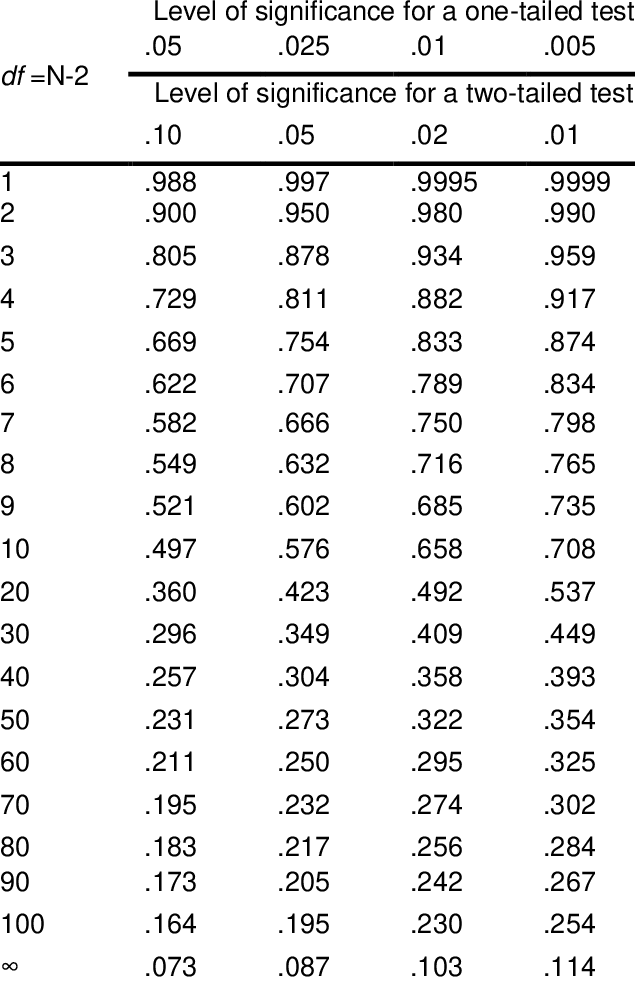
\includegraphics[scale=0.3]{rtable.png}
    \caption{Tabla de valores de $r$ en función de los grados de libertad}
  \end{center}
\end{figure}

En este caso tenemos 8 grados de libertad debido a que el tamaño de la  $N$ es de 10. Si seguimos en la tabla el renglón de 8 grados de libertad y buscamos el valor más aproximado al resultado de $r = -0.95$ obtenido (pero sin pasarnos de él), encontraremos que el resultado es significativo al nivel de 0.01 para una prueba de dos colas, es decir, que en una población en la cual no existiese ninguna relación entre las manzanas y las visitas al médico encontraríamos un coeficiente de correlación de -0.95 en menos de 1 de cada 100 muestras con $N = 10$ tomadas. Un nivel muy razonable de confianza.

\section{Diferencia entre grupos}\label{diferenciaentregrupos}

Además de el cambio coordinado entre dos variables es posible determinar el cambio entre dos grupos expuestos a manipulaciones distintas, o más precisamente, a dos niveles de una manipulación. El caso más simple fue el visto con la prueba $z$ en el cual comparamos el grupo experimental con el nivel ya conocido de la población de la que se toma la muestra. Sin embargo, casos así serán la excepción más que la regla debido a que es difícil conocer las características reales de poblaciones completas (a no ser que se obtengan datos de un censo poblacional). Lo más común será que tomemos dos muestras de una población con características desconocidas, establezcamos manipulaciones distintas, y debamos hacer una comparación entre ellas para determinar si las manipulaciones son eficaces para modificar las características de las poblaciones.

En un experimento con dos muestras medimos las puntuaciones de los sujetos bajo dos condiciones. La condición 1 produce una ${\bar{X}}$ que representa a $\mu_{1}$, la $\mu$ que encontraríamos si se le aplicara la manipulación a toda la población. Del mismo modo, la condición 2 produce una $\mu_{2}$. Un resultado posible sería el siguiente:

\begin{tikzpicture}
  \begin{axis}[
    no markers, domain=-4:6, samples=100,
    axis lines*=left,
    height=5cm, width=12cm,
    xtick=\empty, ytick=\empty,
    enlargelimits=false, clip=false, axis on top,
    grid = major
    ]
    \addplot [very thick,cyan!50!black] {gauss(0,1)};
    \addplot [very thick,cyan!50!black] {gauss(3,1)};
    \draw [very thick, white!20!black] (0, 0) -- (0, 0.4) node [anchor=south] {$\mu_{1}$};
    \draw [very thick, white!20!black] (3, 0) -- (3, 0.4) node [anchor=south] {$\mu_{2}$};
  \end{axis}
\end{tikzpicture}

Idealmente podríamos concluir que, si las medias poblacionales $\mu$ representadas por las medias muestrales $\bar{X}$ son distintas, entonces la manipulación tiene un efecto. Pero, de nuevo, la realidad no es tan bella. Existe también aquí la posibilidad de un error de muestreo que genere la diferencia: quizá desde el comienzo, antes de la manipulación, las muestras ya tenían medias distintas por azar a pesar de estar representando a una misma población. Siendo así, es necesario demostrar que la diferencia encontrada entre las medias de las muestras es lo bastante grande para poder afirmar con niveles razonables de seguridad que no pertenecen a una misma población. Ese es el papel de la prueba T.

El principio estadístico es similar al principio de la prueba $z$: es necesario determinar la posición de un resultado dentro de una distribución muestral. Sin embargo, debido a que estamos determinando si una diferencia entre medias es {\slshape significativa}, es necesario que la distribución muestral esté también en términos de diferencias entre medias.

En esta ocasión suponemos una cantidad infinita de {\slshape pares} de muestras tomados de una población. Para cada par calculamos la media de cada uno y los restamos entre sí. El proceso se repite infinitamente y las diferencias entre las medias de las muestras se grafican en un histograma de frecuencias. Al graficar nos daremos cuenta de que las diferencias entre infinitas medias tomadas de una misma población tienden a formar una distribución normal, es decir, que también son descritas por el teorema central del límite (figura 3).

\begin{figure}[!ht]
  \begin{center}
    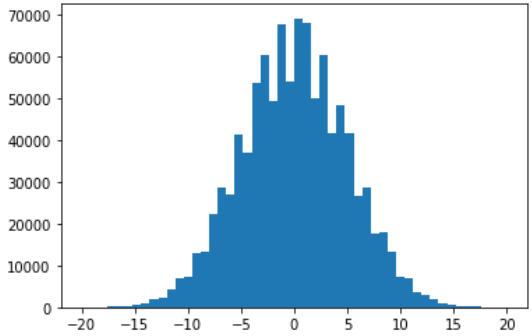
\includegraphics[scale=0.5]{diferenciaMedias.png}
  \end{center}
\end{figure}

La única diferencia con el histograma que ya conocemos es que en esta ocasión, debido a que estamos calculando diferencias entre medias de una misma población, los datos se agruparán alrededor del valor de 0. Esto se debe a que frecuentemente se muestrearán valores cercanos a la media real de la población, y restarlos entre sí generalmente resultará en números pequeños. Solo en las pocas ocasiones en que se muestreen valores muy alejados de la media poblacional se encontrarán valores altos para la diferencia entre las medias.

La prueba T tiene como función determinar en qué posición de la distribución de {\slshape diferencias de medias} se encuentra el valor que encontramos en un estudio dado. Si ese valor se encuentra lo bastante lejos de la distribución como para ser muestreado en menos del 5\% de las ocasiones (o lo que determinemos con el umbral $\alpha$), entonces determinaremos que existen diferencias entre nuestros grupos, pues será improbable que un valor elevado provenga de una distribución de {\slshape diferencias de medias} centrada en 0.

La prueba T tiene dos variantes:
\begin{itemize}
  \item Para muestras independientes: se usa si los sujetos de cada grupo son muestreados sin tomar en cuenta a los del otro grupo.
  \item Para muestras relacionadas: se usa si los datos de ambos grupos provienen de los mismos sujetos pasando por condiciones distintas, o si los sujetos fueron seleccionados de manera propositiva mediante pareo.
\end{itemize}

La prueba T para muestras independientes tiene como requisitos:
\begin{enumerate}
  \item Los puntajes tienen nivel de intervalo o razón
  \item Las poblaciones tienen distribuciones aproximadamente normales
  \item Las poblaciones tienen varianzas homogéneas, es decir, que si computamos la varianza de cada población por separado obtendríamos el mismo resultado.
  \item La cantidad $n$ de casos es similar
\end{enumerate}

Las hipótesis estadísticas en este caso están dichas en términos de las diferencias entre las medias de las poblaciones de las cuales vienen las muestras. Es decir, la hipótesis alternativa indicaría que la media poblacional $\mu_{1}$ es {\slshape distinta} de la media poblacional $\mu_{2}$:
\[
  H_{a}: \mu_{1} \neq \mu_{2}
,\]
o en términos de su diferencia:
\[
  H_{a}: \mu_{1} - \mu_{2} \neq 0
.\]
La hipótesis nula diría que su diferencia sí es de cero:
\begin{eqnarray*}
  H_{0}: \mu_{1} = \mu_{2}\\
  H_{0}: \mu_{1} - \mu_{2} = 0
\end{eqnarray*}

Las hipótesis no tienen un valor específico para $\mu$, por lo que serán las mismas para cualquier estudio.

La manera de contrastar las hipótesis es calculando el valor de $t$, un estadístico que indica la posición de la diferencia entre las medias dentro de la distribución de diferencias dada por el teorema central del límite.

La fórmula del estadístico $t$ es:
\[
  t_{obt} = \frac{
    (\bar{X}_{1} - \bar{X}_{2}) - (\mu_{1} - \mu_{2})
  }{
    s_{\bar{X}_{1} - \bar{X}_{2}}
  }
\]
Se trata de una fórmula similar a la del puntaje $z$ debido a que su significado es similar: la posición del valor obtenido con respecto a una distribución normal. Se obtiene la diferencia entre {\slshape la diferencia entre medias muestrales} y {\slshape la diferencia entre medias poblacionales} (así es, una diferencia de diferencias), y el resultado se divide entre un error estándar. El valor $s_{\bar{X}_{1} - \bar{X}_{2}}$ se refiere al {\slshape error estándar de la diferencia}, es decir, qué tanto se alejan en promedio las diferencias entre medias muestreadas del valor central de la distribución. La forma de calcularlo es la siguiente:
\[
  s_{\bar{X}_{1} - \bar{X}_{2}} =\sqrt{
    \left(s_{pool}^{2}\right)\left(\frac{1}{n_{1}} + \frac{1}{n_{2}}\right)
  }
.\]
Finalmente, en esta última fórmula el valor $s_{pool}^{2}$ se refiere a la {\slshape varianza agrupada}, que es la media ponderada de varianzas. Específicamente, esto se refiere a la media de las varianzas de las dos poblaciones de las que provienen los datos, pero con un peso asignado en función de la cantidad de datos que tiene cada grupo usando los grados de libertad de cada muestra:
\[
  s_{pool}^{2} = \frac{
    (n_{1} - 1)s_{1}^{2} + (n_{2} - 1)s_{2}^{2}
  }{
    (n_{1} - 1) + (n_{2} - 1)
  }
\]

Así, la forma de calcular $t$ es:
\begin{enumerate}
  \item Obtener la varianza agrupada
  \item Obtener el error estándar de las diferencias
  \item Calcular el estadístico $t$
\end{enumerate}

El valor resultante de $t_{\mbox{\scriptsize obtenida}}$ se compara con una tabla de valores críticos y eso permite determinar la significancia de la prueba.

{\noindent\scshape\bfseries Ejemplo}

Se pretende determinar si acaso hay diferencias entre los perros border collie y los golden retriever en la capacidad de aprender y recordar nombres de objetos. Para ello se seleccionan perros de cada raza al azar y se les enseña, a lo largo de una semana, a traer 30 juguetes tras escuchar su nombre. Después de una semana se hace una prueba para determinar cuántos nombres recuerdan aun. Supongamos que se encontraron 17 perros collie y 15 retriever. En promedio los collie recordaron 23 comandos; y los retriever, 20. La varianza del grupo de collie es de 9, y la del grupo de retriever es de 7.5. Nuestra labor es determinar si los collie son mejores para recordar comandos con base en los datos de nuestra muestra.

Como primer paso obtenemos la diferencia entre las medias de los grupos:
\[
  23 - 20 = 3
,\]
es decir, la diferencia en puntaje entre grupos es de 3.

Primero estimamos la varianza agrupada. Recordamos que la fórmula es:
\begin{eqnarray*}
  s_{pool}^{2}&=&\frac{
    (n_{1} - 1)s_{1}^{2} + (n_{2} - 1)s_{2}^{2}
  }{
    (n_{1} - 1) + (n_{2} - 1)
  }\\[3mm]
  &=& \frac{
    (17 - 1) 9 + (15 - 1) 7{.}5
  }{
    (17 - 1) + (15 - 1)
  }\\[3mm]
  &=& \frac{
    144 + 105
  }{
    30
  }\\[3mm]
  &=& \frac{
    249
  }{
    30
  }\\[3mm]
  &=& 8{.}3
\end{eqnarray*}
Así estimamos que la varianza conjunta de la población de ambas razas de perros es de 8.3.

Después utilizamos la varianza agrupada para calcular el error estándar de la diferencia:
\begin{eqnarray*}
  s_{\bar{X}_{1} - \bar{X}_{2}}&=&\sqrt{
  \left(s_{pool}^{2}\right)\left(\frac{1}{n_{1}} + \frac{1}{n_{2}}\right)}\\[3mm]
  &=& \sqrt{
    8{.}3\left(\frac{1}{17} + \frac{1}{15}\right)
  }\\[3mm]
  &=& \sqrt{8{.}3(0{.}126)}\\[3mm]
  &=& \sqrt{1{.}046}\\
  &=& 1{.}023
\end{eqnarray*}
El error estándar de la diferencia es entonces de 1.023. Finalmente esto es utilizado para calcular el estadístico $t$:
\begin{eqnarray*}
  t_{\mbox{\scriptsize obtenida}}&=&\frac{
    (\bar{X}_{1} - \bar{X}_{2}) - (\mu_{1} - \mu_{2})
  }{
    s_{\bar{X}_{1} - \bar{X}_{2}}
  }\\[3mm]
  &=&\frac{
    (23 - 20) - 0
  }{
    1{.}023
  }\\[3mm]
  &=&\frac{
    (+3{.}0) - 0
  }{
    1{.}023
  }\\[3mm]
  &=&+2{.}93
\end{eqnarray*}

El valor $t = +2{.}93$ nos indica la posición de la distribución de diferencias de medias en la cual se ubica nuestra diferencia medida de +3. Para interpretar este valor es necesario compararlo con una tabla de valores críticos de $t$. Es necesaria una tabla debido a que para cada cantidad de grados de libertad, el histograma de frecuencias de diferencias de medias tiene una forma ligeramente distinta, así que para distintos grados de libertad cada punto de $t$ estará en una localización ligeramente distinta.

En este caso tenemos un tamaño de $N$ de 32, y la manera de calcular los grados de libertad para una prueba $t$ es:
\[
gl = N - 2
\]
debido a que se tienen dos grupos. Sustituyendo con los valores del ejemplo:
\[
gl = 32 -2 = 30
\]
\begin{figure}[!ht]
  \begin{center}
    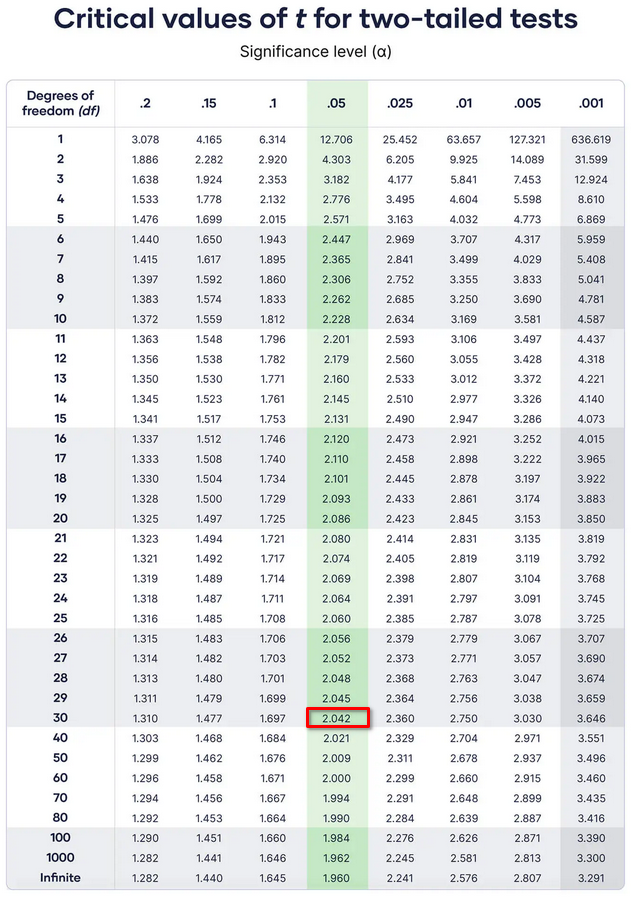
\includegraphics[scale=0.5]{tablaT.png}
  \end{center}
\end{figure}

Con un $\alpha = 0{.}05$ y una prueba de dos colas, el valor crítico de $t$ es de $\pm 2{.}042$. El valor obtenido está más allá de este punto, por lo que podemos concluir que la diferencia encontrada en la muestra es significativa, es decir, que difícilmente sería encontrada si acaso no existiese una relación entre la raza de perro y la capacidad para recordar comandos.


\end{document}
